%%%%%%%%%%%%%%%%%%%%%%%%%%%%%%%%%%%%%%%%%
% University/School Laboratory Report
% LaTeX Template
% Version 4.0 (March 21, 2022)
%
% This template originates from:
% https://www.LaTeXTemplates.com
%
% Authors:
% Vel (vel@latextemplates.com)
% Linux and Unix Users Group at Virginia Tech Wiki
%
% License:
% CC BY-NC-SA 4.0 (https://creativecommons.org/licenses/by-nc-sa/4.0/)
%
%%%%%%%%%%%%%%%%%%%%%%%%%%%%%%%%%%%%%%%%%

%----------------------------------------------------------------------------------------
%	PACKAGES AND DOCUMENT CONFIGURATIONS
%----------------------------------------------------------------------------------------

\documentclass[
	letterpaper, % Paper size, specify a4paper (A4) or letterpaper (US letter)
	11pt, % Default font size, specify 10pt, 11pt or 12pt
]{CSUniSchoolLabReport}

\usepackage{subcaption}
\usepackage{booktabs}
\geometry{top=2cm} % Override top margin to reduce space before title

%----------------------------------------------------------------------------------------
%	REPORT INFORMATION
%----------------------------------------------------------------------------------------

\title{Lab 2 - Electric Flux} % Report title

\author{Yiran \textsc{Liu} \&  Zijin \textsc{Yang}} % Author name(s), add additional authors like: '\& James \textsc{Smith}'

%----------------------------------------------------------------------------------------

\begin{document}

\maketitle % Insert the title, author and date using the information specified above

\begin{center}
	\begin{tabular}{l r}
      ECE 106: 	Electricity and Magnetism \\
      Student Number: Y.L. 21184901 \& Z.Y. 21196273
	\end{tabular}
\end{center}
%----------------------------------------------------------------------------------------
%	COMPUTATIONS
%----------------------------------------------------------------------------------------

\section{Theory}

We consider the system of two spherical uniform charges ($a=0.01m$, $Q=+1.0 \mu C$) placed $r=0.2m$ apart. We compute the total electrical energy:

\[
  W_\text{total} = n \times W_\text{formation} + W_\text{assembly} = 2 \times \frac{3}{5} \frac{Q^2}{4\pi \epsilon_0 a} + \frac{1}{4} \frac{Q^2}{r} = 1.1234 J
\]

\section{System of two like charges}
We build the simulation model of two point charges ($R=0.01$ and $Q=+1.0 \mu C$) located at $(0, 0, 0)$ and $(0.2, 0.0, 0.0)$ with zero volts boundary condition at $R = 50.0m$ in COMSOL. We compare the evaluated value with theoretical:

\begin{figure}[H] % [H] forces the figure to be placed exactly where it appears in the text
	\centering % Horizontally center the figure
	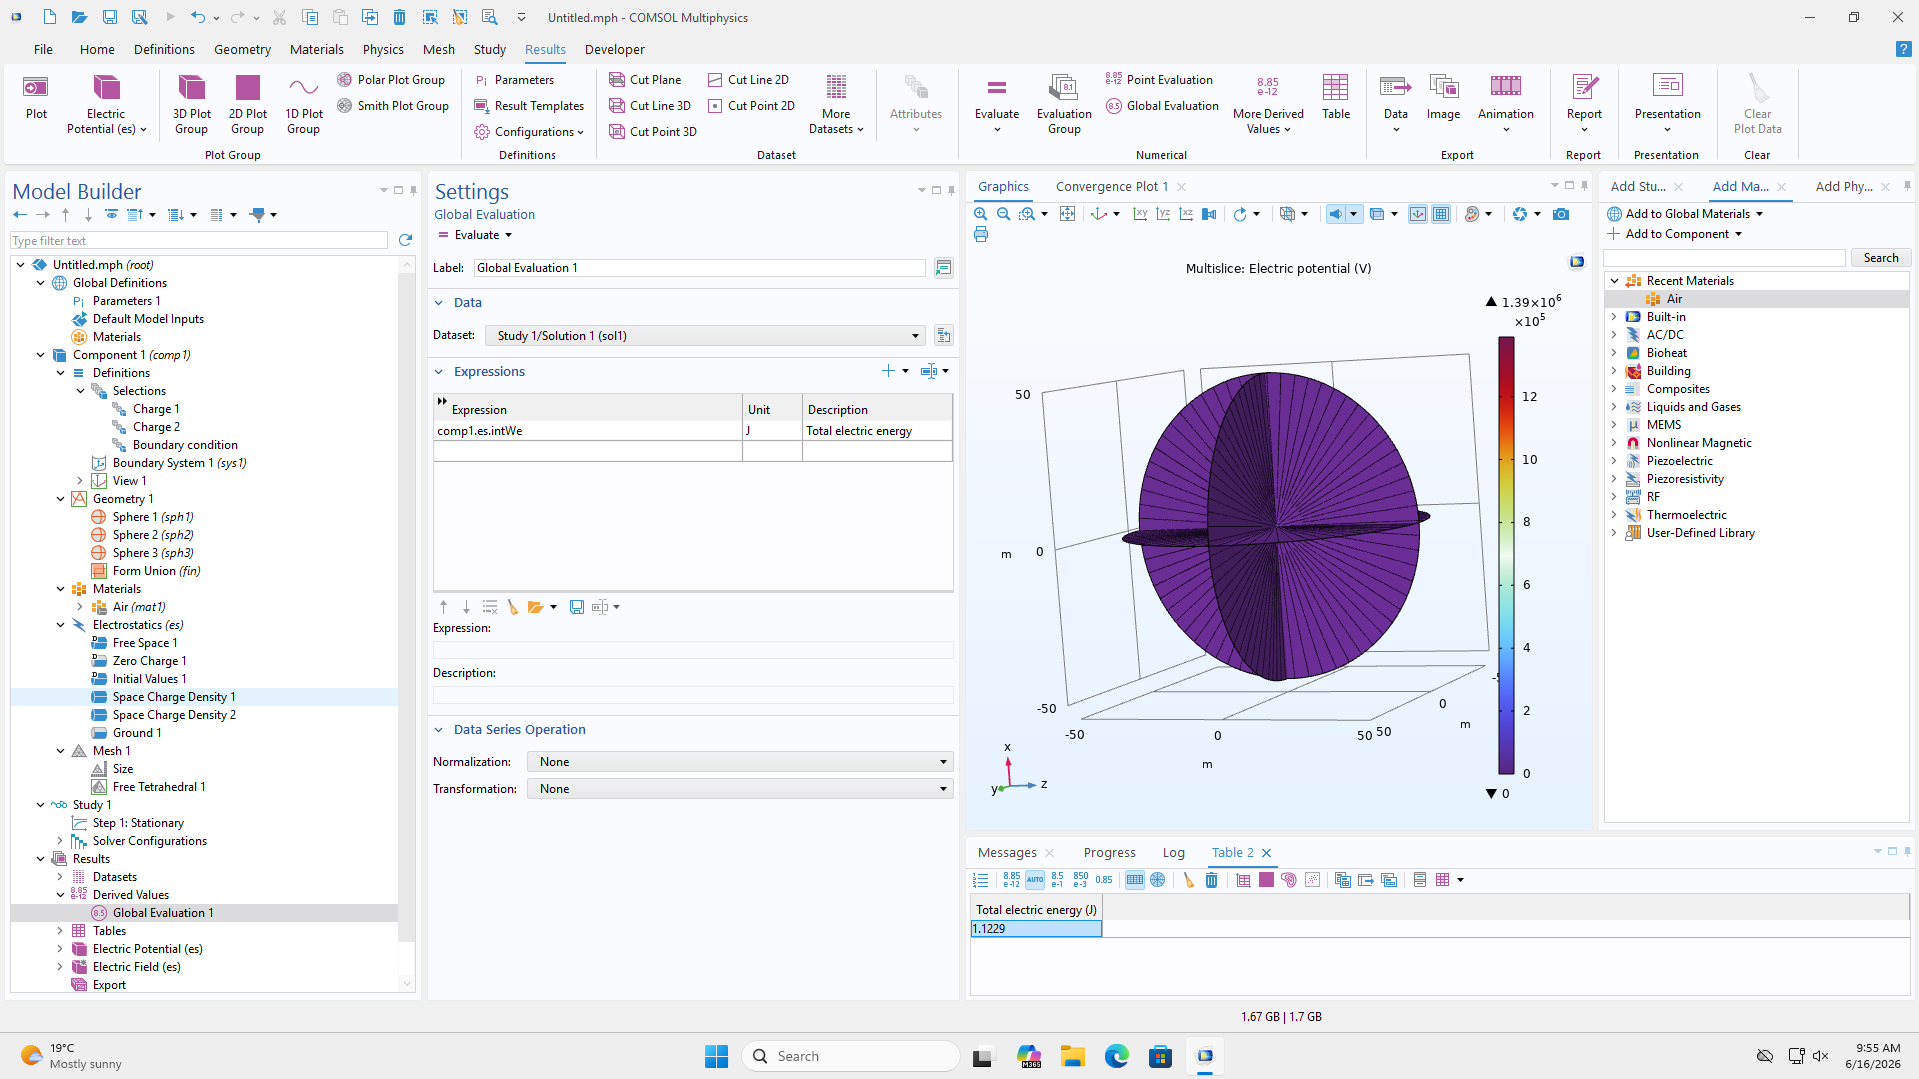
\includegraphics[width=0.8\textwidth]{./figures/two_like_charges_energy} % Include the figure
  \caption{Energy in system of two like charges measured in COMSOL.}
\end{figure}

\begin{table}[H]
    \centering
    \begin{tabular}{lcrr}
        \toprule
        \textbf{Simulated} ($J$) & \textbf{Theoretical} ($J$) & \textbf{\% Error} \\
        \midrule
        1.2229 & 1.1234 & 0.0484\% \\
        \bottomrule
    \end{tabular}
\end{table}

\begin{figure}[H] % [H] forces the figure to be placed exactly where it appears in the text
	\centering % Horizontally center the figure
	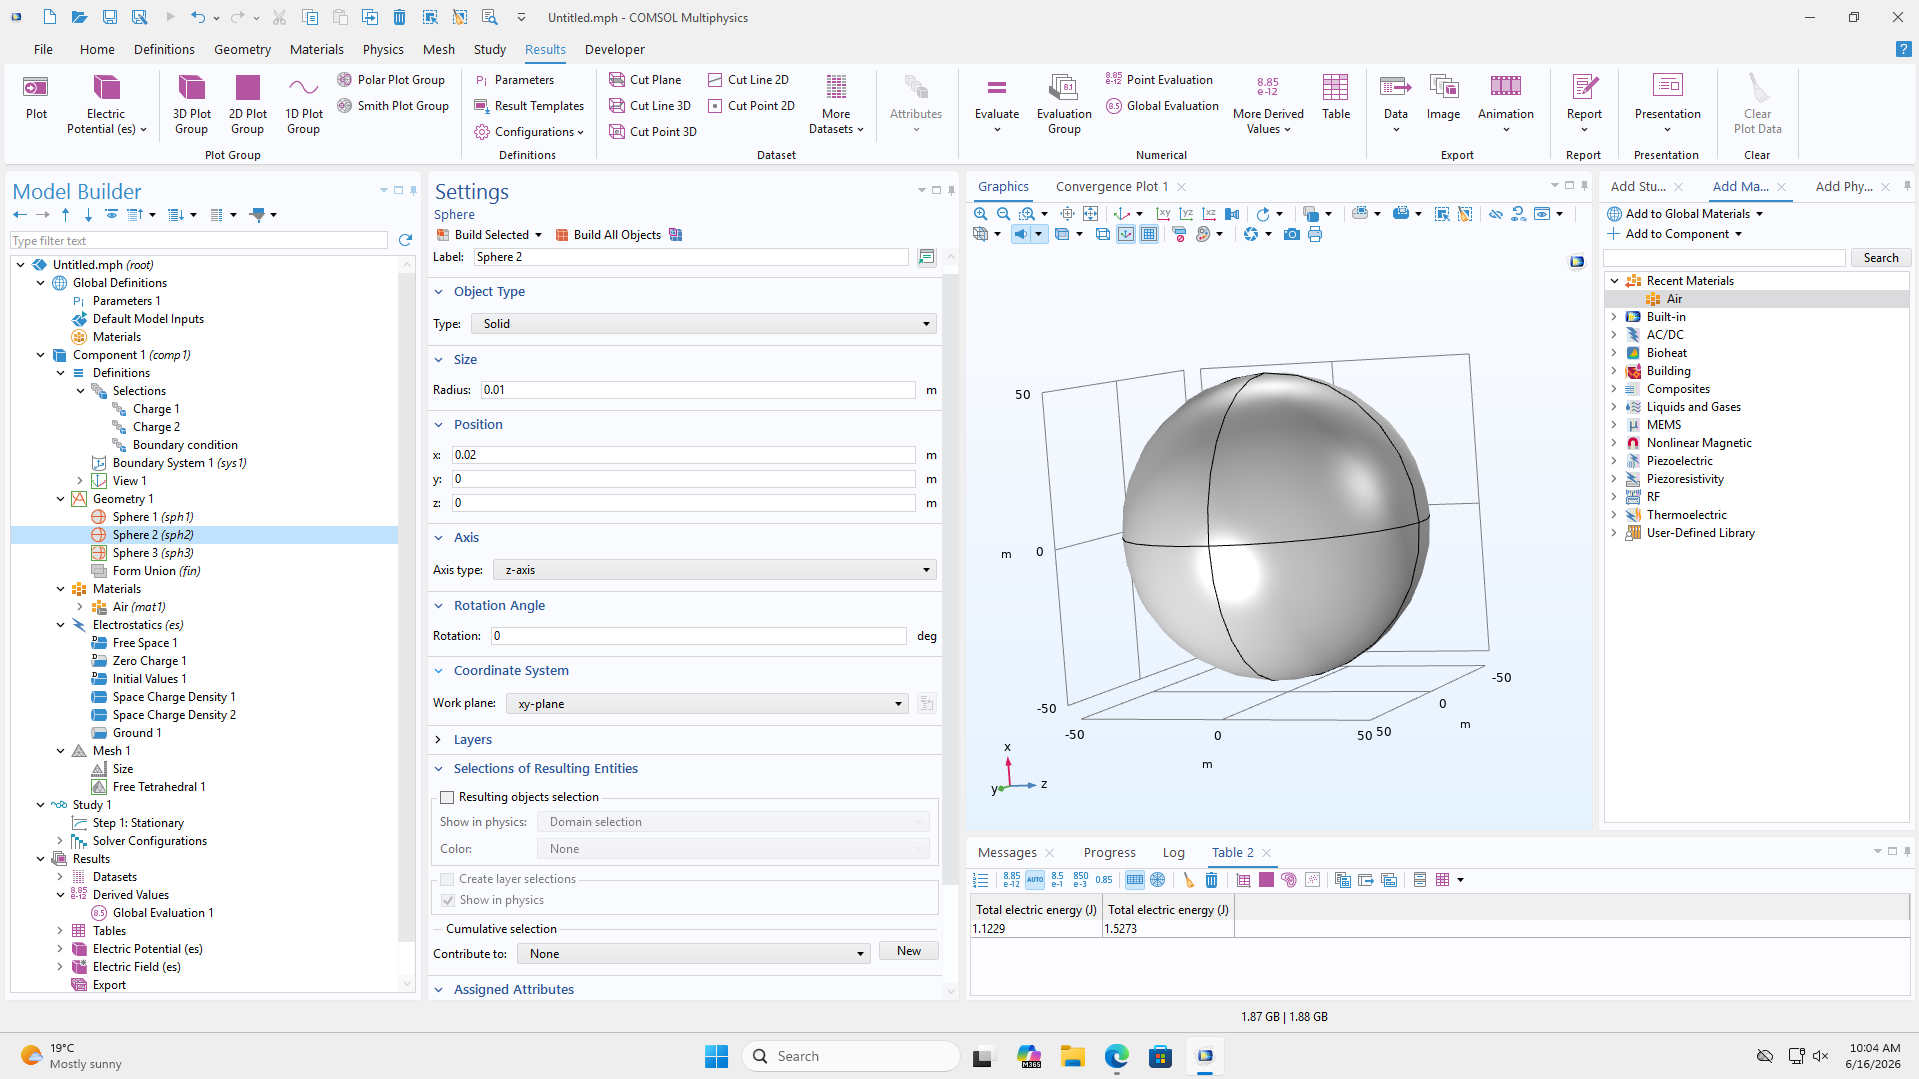
\includegraphics[width=\textwidth]{./figures/two_like_charges_energy_increased} % Include the figure
  \caption{Energy in system of two like charges, increased (right in table).}
\end{figure}

\section{System of two opposite charges}
We build the simulation model of two opposite charges.

\begin{figure}[H] % [H] forces the figure to be placed exactly where it appears in the text
	\centering % Horizontally center the figure
	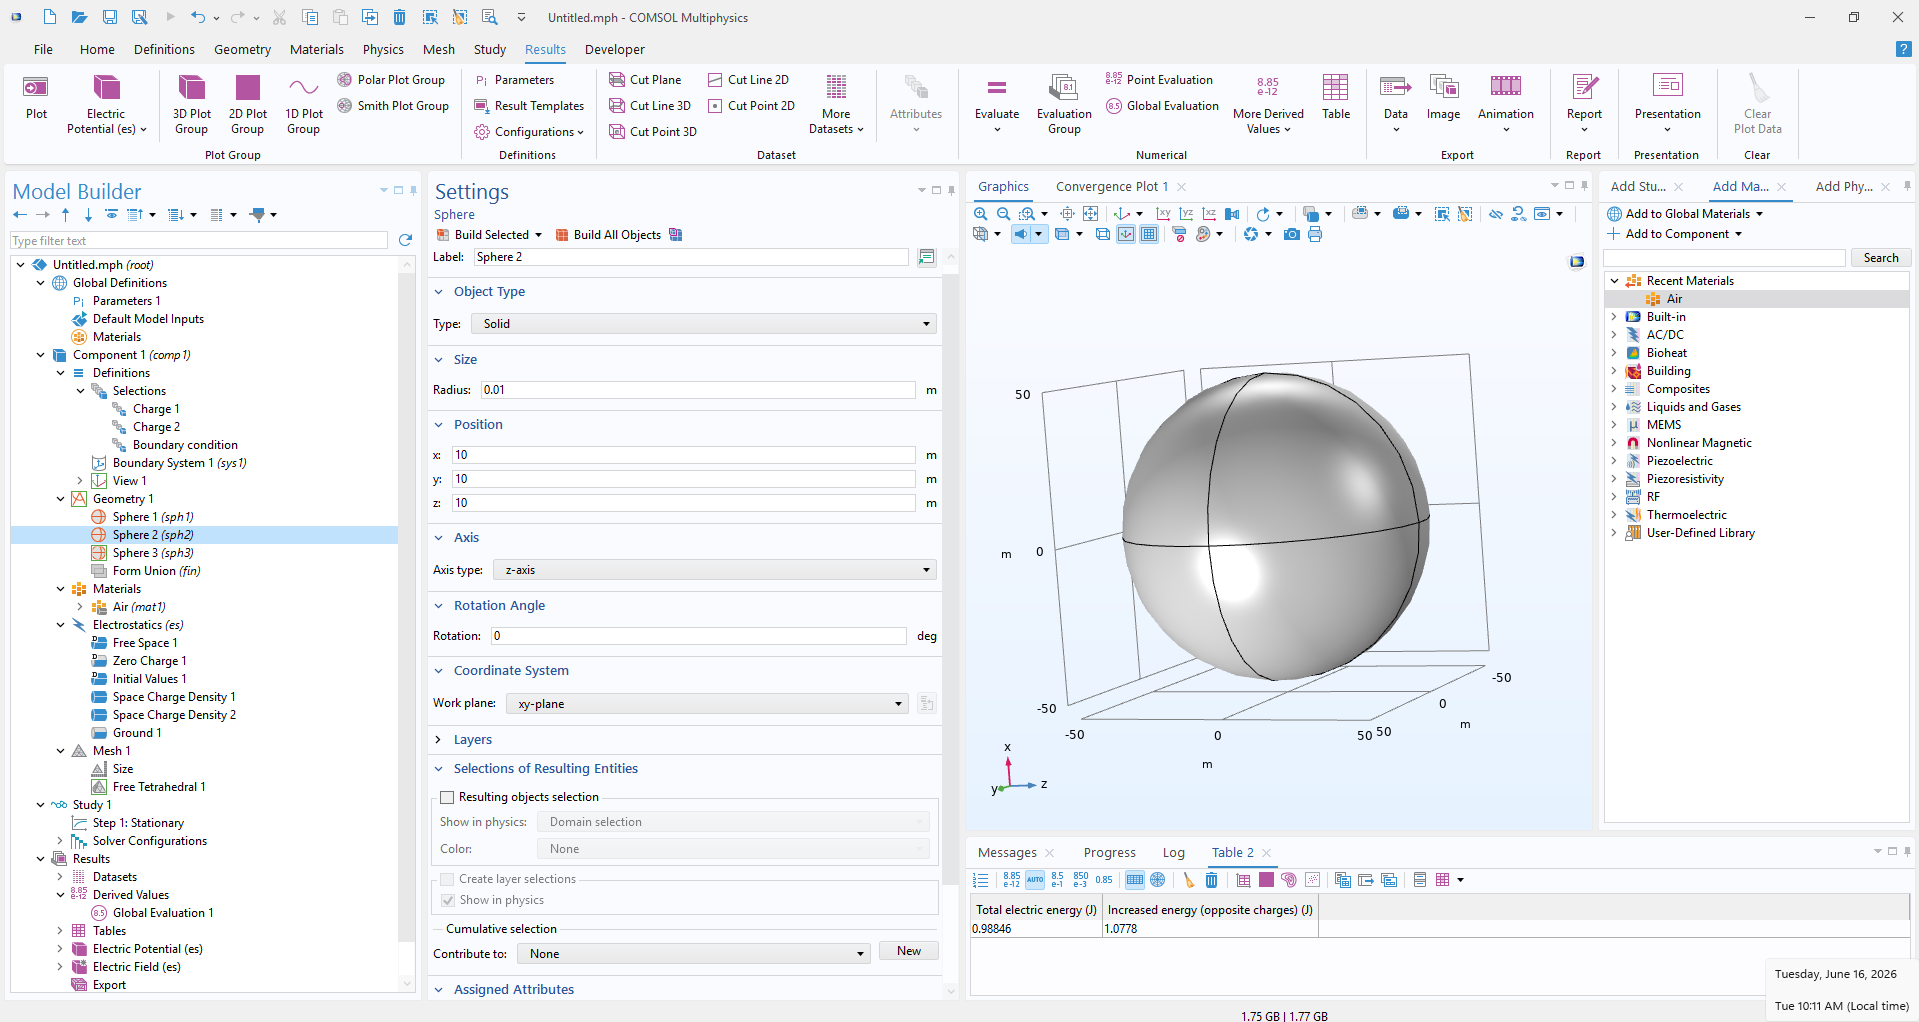
\includegraphics[width=\textwidth]{./figures/opposite_charges_energy_increased.png} % Include the figure
  \caption{Energy in the system of two opposite charges (left in table) compared to increased value (right in table). }
\end{figure}

\section{Analysis of Electric Potential}


\end{document}